\documentclass[10pt,a4paper]{article}

%%%%%%%%%%%%%%%%%%%%%%%%%%%%%%%%%%%%%%%%%%%%%%%%%%%%%%%%%%%%
% PACKAGES
%%%%%%%%%%%%%%%%%%%%%%%%%%%%%%%%%%%%%%%%%%%%%%%%%%%%%%%%%%%%

\usepackage{fontspec}
\usepackage{xcolor}
\usepackage{pagecolor}
\usepackage{tikz}
\usepackage{geometry}
\usepackage{graphicx}
\usepackage{eso-pic}
\usepackage{enumitem}
\usepackage{hyperref}

\pgfmathsetseed{42}

\usetikzlibrary{
calc,
positioning,
backgrounds,
shadows.blur,
decorations.pathmorphing
}

%%%%%%%%%%%%%%%%%%%%%%%%%%%%%%%%%%%%%%%%%%%%%%%%%%%%%%%%%%%%
% PAGE
%%%%%%%%%%%%%%%%%%%%%%%%%%%%%%%%%%%%%%%%%%%%%%%%%%%%%%%%%%%%

\geometry{
left=1.4cm,
right=1.4cm,
top=1.4cm,
bottom=1.4cm
}

\pagecolor{black}
\color{white}

%%%%%%%%%%%%%%%%%%%%%%%%%%%%%%%%%%%%%%%%%%%%%%%%%%%%%%%%%%%%
% FONTS
%%%%%%%%%%%%%%%%%%%%%%%%%%%%%%%%%%%%%%%%%%%%%%%%%%%%%%%%%%%%

\setmainfont{TeX Gyre Termes}

\newfontfamily\displayfont{TeX Gyre Heros}
\newfontfamily\monofont{TeX Gyre Cursor}

%%%%%%%%%%%%%%%%%%%%%%%%%%%%%%%%%%%%%%%%%%%%%%%%%%%%%%%%%%%%
% COLORS
%%%%%%%%%%%%%%%%%%%%%%%%%%%%%%%%%%%%%%%%%%%%%%%%%%%%%%%%%%%%

\definecolor{fog}{HTML}{A8DADC}
\definecolor{deepwater}{HTML}{0B132B}
\definecolor{coast}{HTML}{1C2541}
\definecolor{plateau}{HTML}{3A506B}
\definecolor{ridge}{HTML}{5BC0BE}
\definecolor{peak}{HTML}{F4D35E}
\definecolor{accent}{HTML}{EE6C4D}

%%%%%%%%%%%%%%%%%%%%%%%%%%%%%%%%%%%%%%%%%%%%%%%%%%%%%%%%%%%%
% BACKGROUND ART
%%%%%%%%%%%%%%%%%%%%%%%%%%%%%%%%%%%%%%%%%%%%%%%%%%%%%%%%%%%%

\AddToShipoutPictureBG{

\begin{tikzpicture}[remember picture,overlay]

%%%%%%%%%%%%%%%%%%%%%%%%%%%%%%%%%%%%%%%%
% ATMOSPHERIC GLOW
%%%%%%%%%%%%%%%%%%%%%%%%%%%%%%%%%%%%%%%%

\shade[
inner color=deepwater,
outer color=black
]
(current page.center)
circle (18cm);

%%%%%%%%%%%%%%%%%%%%%%%%%%%%%%%%%%%%%%%%
% TOPOGRAPHICAL TERRAIN
%%%%%%%%%%%%%%%%%%%%%%%%%%%%%%%%%%%%%%%%

\foreach \i in {1,...,40}
{
\begin{scope}[xshift=\i*0.8pt]

\draw[
ridge,
opacity=.05,
line width=.5pt
]
plot[smooth cycle]
coordinates{
(2,8)
(4,9)
(8,8.7)
(11,7.8)
(12,5.5)
(11,3)
(9,1)
(6,.8)
(3,2)
};

\end{scope}
}

%%%%%%%%%%%%%%%%%%%%%%%%%%%%%%%%%%%%%%%%
% NOISE FIELD
%%%%%%%%%%%%%%%%%%%%%%%%%%%%%%%%%%%%%%%%

\foreach \i in {1,...,250}
{
\pgfmathsetmacro{\nx}{rnd*21}
\pgfmathsetmacro{\ny}{rnd*29}
\pgfmathsetmacro{\nr}{0.03 + rnd*0.12}

\begin{scope}
\fill[fog, opacity=.015]
(\nx,\ny)
circle (\nr);
\end{scope}
}

%%%%%%%%%%%%%%%%%%%%%%%%%%%%%%%%%%%%%%%%
% LARGE TRANSPARENT LANDMASSES
%%%%%%%%%%%%%%%%%%%%%%%%%%%%%%%%%%%%%%%%

\fill[
plateau,
opacity=.10
]

(2,17)
.. controls (5,24) and (9,24)
.. (12,18)
.. controls (14,12) and (11,8)
.. (6,9)
.. controls (2,10) and (1,13)
.. cycle;

\fill[
ridge,
opacity=.07
]

(9,8)
.. controls (12,11) and (15,10)
.. (17,7)
.. controls (18,4) and (14,2)
.. (11,4)
.. cycle;

%%%%%%%%%%%%%%%%%%%%%%%%%%%%%%%%%%%%%%%%
% DEPTH SHADOWS
%%%%%%%%%%%%%%%%%%%%%%%%%%%%%%%%%%%%%%%%

\fill[
black,
opacity=.22
]
plot[smooth cycle, tension=1]
coordinates{
(2.3,16.5)
(5.3,23.5)
(9.3,23.5)
(12.3,17.5)
(14.3,11.5)
(11.3,7.5)
(6.3,8.5)
(2.3,9.5)
(1.3,12.5)
};

%%%%%%%%%%%%%%%%%%%%%%%%%%%%%%%%%%%%%%%%
% FLOATING LABELS
%%%%%%%%%%%%%%%%%%%%%%%%%%%%%%%%%%%%%%%%

\node[
scale=9,
rotate=12,
text opacity=.035,
color=peak
]
at (current page.center)
{
TERRAIN
};

\node[
scale=7,
rotate=-22,
text opacity=.03,
color=ridge
]
at ($(current page.center)+(0,-6)$)
{
NETWORK
};

%%%%%%%%%%%%%%%%%%%%%%%%%%%%%%%%%%%%%%%%
% ATMOSPHERIC HAZE
%%%%%%%%%%%%%%%%%%%%%%%%%%%%%%%%%%%%%%%%

\foreach \i in {1,...,18}
{
\fill[
white,
opacity=.004
]

(current page.center)
circle (\i*0.9cm);
}

\end{tikzpicture}
}

%%%%%%%%%%%%%%%%%%%%%%%%%%%%%%%%%%%%%%%%%%%%%%%%%%%%%%%%%%%%
% SECTION STYLE
%%%%%%%%%%%%%%%%%%%%%%%%%%%%%%%%%%%%%%%%%%%%%%%%%%%%%%%%%%%%

\newcommand{\terrainsection}[1]
{

\vspace{1em}

{\Huge
\displayfont
\bfseries
\textcolor{peak}{#1}
}

\vspace{0.2em}

{\color{ridge}
\rule{\linewidth}{1pt}
}

\vspace{0.5em}

}

%%%%%%%%%%%%%%%%%%%%%%%%%%%%%%%%%%%%%%%%%%%%%%%%%%%%%%%%%%%%
% ENTRY
%%%%%%%%%%%%%%%%%%%%%%%%%%%%%%%%%%%%%%%%%%%%%%%%%%%%%%%%%%%%

\newcommand{\landmark}[4]
{

\vspace{0.6em}

{\Large\bfseries\color{accent} #1}
\hfill
{\color{fog} #2}

\vspace{0.2em}

{\itshape\color{peak} #3}
\hfill
{\color{ridge} #4}

\vspace{0.3em}

}

%%%%%%%%%%%%%%%%%%%%%%%%%%%%%%%%%%%%%%%%%%%%%%%%%%%%%%%%%%%%
% DOCUMENT
%%%%%%%%%%%%%%%%%%%%%%%%%%%%%%%%%%%%%%%%%%%%%%%%%%%%%%%%%%%%

\begin{document}

%%%%%%%%%%%%%%%%%%%%%%%%%%%%%%%%%%%%%%%%
% HEADER
%%%%%%%%%%%%%%%%%%%%%%%%%%%%%%%%%%%%%%%%

\vspace*{1cm}

{\displayfont

{\fontsize{42}{42}\selectfont
\color{peak}
JANE DOE

}

\vspace{0.2cm}

{\Large
\color{ridge}
Infrastructure Cartographer
}

\vspace{0.2cm}

{\monofont
\color{fog}
gothenburg
|
(+46)72222222
|
mom@gmail.com
}

}

\vspace{1.5cm}

%%%%%%%%%%%%%%%%%%%%%%%%%%%%%%%%%%%%%%%%
% EDUCATION
%%%%%%%%%%%%%%%%%%%%%%%%%%%%%%%%%%%%%%%%

\terrainsection{Education}

\landmark
{IT Högskolan}
{Stockholm}
{Higher Vocational Degree in Penetration Testing}
{2026}

%%%%%%%%%%%%%%%%%%%%%%%%%%%%%%%%%%%%%%%%
% EXPERIENCE
%%%%%%%%%%%%%%%%%%%%%%%%%%%%%%%%%%%%%%%%

\terrainsection{Expeditions}

\landmark
{Enclave AB}
{Remote}
{Infrastructure Lead Developer}
{2025--2026}

Built air-gapped Kubernetes environments, AI-assisted operations and secure cloud-native platforms.

\vspace{0.4cm}

\landmark
{Mekonomen Group}
{Östersund}
{Customer Service Agent}
{2024}

Identified vulnerabilities while studying internal systems and workflows.

\vspace{0.4cm}

\landmark
{Alina Service}
{Östersund}
{Technical Repair Shop Assistant}
{2024}

Hardware diagnostics, refurbishment and software recovery.

%%%%%%%%%%%%%%%%%%%%%%%%%%%%%%%%%%%%%%%%
% SKILLS
%%%%%%%%%%%%%%%%%%%%%%%%%%%%%%%%%%%%%%%%

\terrainsection{Skill Archipelago}

\begin{center}

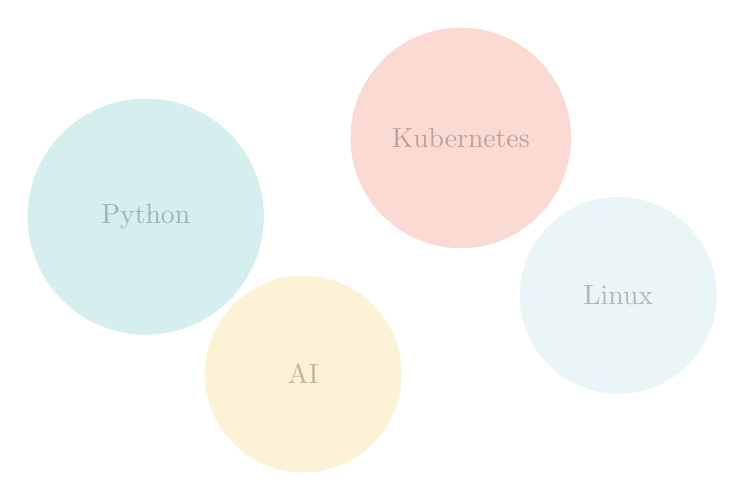
\begin{tikzpicture}

\node[
circle,
fill=ridge,
fill opacity=.25,
minimum size=3cm
]
at (0,0)
{
Python
};

\node[
circle,
fill=accent,
fill opacity=.25,
minimum size=2.8cm
]
at (4,1)
{
Kubernetes
};

\node[
circle,
fill=peak,
fill opacity=.25,
minimum size=2.5cm
]
at (2,-2)
{
AI
};

\node[
circle,
fill=fog,
fill opacity=.25,
minimum size=2.5cm
]
at (6,-1)
{
Linux
};

\end{tikzpicture}

\end{center}

\vfill

\begin{center}

{\Huge
\color{white!20}
MAP OF A DEVELOPING SYSTEM
}

\end{center}

\end{document}
